
Um motor DC é fundamentalmente uma máquina elétrica de corrente contínua, que
converte energia elétrica de corrente contínua em energia mecânica. Máquinas
elétricas de corrente contínua são mais fácies de controlar e oferecem uma
grande faixa de velocidades \cite{Maquinas_eletricas}. Devido a essas
características, tornam-se ótimas candidatas para uso em eletrônica e robótica,
pois podem ser usadas com baterias. Para controlar a velocidade de um motor,
é necessário o uso de um encoder, que converte o sinal de posição em um valor
mensurável de velocidade angular.



\subsection{Encoder magnético}

	Por se utilizar um encoder PRR, são produzidas duas ondas quadradas como saídas,
	A e B \cite{encoder_ppr}. As duas possuem 90° de fase entre si, e, caso a onda A
	esteja adiantada em relação a B (\ref{encoder_ppr_ab}), o sentido de rotação é
	positivo (anti-horário).

\begin{figure}[h]
	\centering
	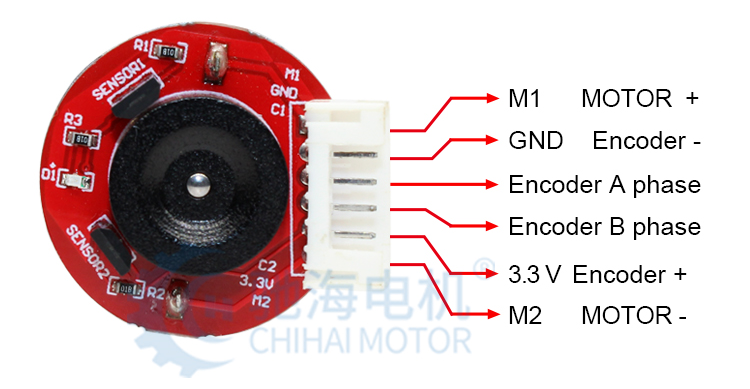
\includegraphics[width=0.6\textwidth]{figures/encoder_holzer}
	\caption{Encoder holzer \cite{motor_dc_6v_encoder}}
\end{figure}

\begin{figure}[h]
	\centering
	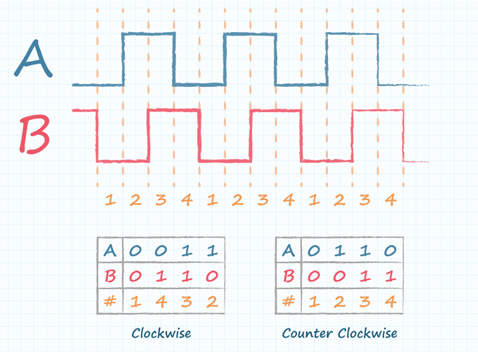
\includegraphics[width=0.6\textwidth]{figures/encoder_pulso_ab}
	\caption{Ondas quadradas resultantes dos pulsos de saída do encoder \cite{encoder_ppr}}
	\label{encoder_ppr_ab}
\end{figure}


\subsection{Driver para motor}

	Motores não podem ser ligados diretamente nos pinos de um microcontrolador -
	é necessário um circuito que permita à baixa corrente do microcontrolador
	controlar correntes mais altas, como as de um motor DC. Drivers podem ser
	usados em uma variedade de tensões de entrada e permitem o controle da
	velocidade por PWM \cite{toshiba_ponte_h}.

	O driver a ser usado neste trabalho é do tipo ponte H. A Ponte H permite que
	a polaridade da alimentação do motor DC seja alterada. Devido a sua inércia,
	o motor continua girando mesmo quando a energia é retirada, mas a ponte H
	pode curto-circuitar seus terminais, gerando uma força eletromotriz de
	frenagem. Outra razão para uso de um driver ponte , é lidar com a tensão
	gerada pelo motor quando o rotor continua a girar depois de remover
	alimentação - o motor se comporta com um gerador nesse momento, e a ponte H
	fornece um caminho livre para essa corrente gerada.


